\documentclass{standalone}
\makeatletter\AtBeginDocument{\@buildstepset{1,2,3,4,5,6,7,8,9,10}}\makeatother
\usepackage{tikz}
\usetikzlibrary{intersections,calc}
\usepackage{hsbcommon}
    \begin{document}
    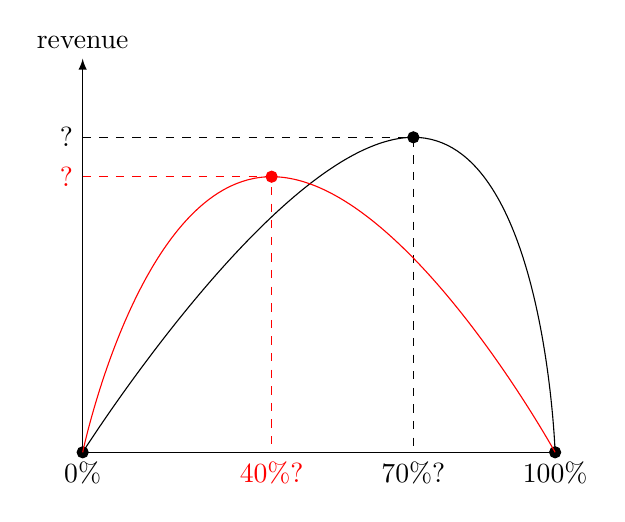
\begin{tikzpicture}

        \draw (0,0) node[below] {$0\%$} -- (6,0) node[below] {$100\%$};
        \draw[->,>=latex] (0,0) -- (0,5) node[above] {revenue};

        \coordinate (A) at (0,0); 
        \coordinate (B) at ({6*7/10},4);
        \coordinate (C) at (6,0);

        \draw  plot [smooth,tension=1] coordinates {(A) (B) (C)};
        
        \filldraw (A) circle (2pt);
        \filldraw (B) circle (2pt);
        \filldraw (C) circle (2pt);
        
        \draw[dashed] (0, |- B) node[left] {?} -- (B) -- (B |-, 0) node[below] {$70\%?$};

        \ifstep{1}{
    \begin{scope}[color=red]

            \coordinate (B2) at ({6*4/10},3.5);
    
            \draw  plot [smooth,tension=1] coordinates {(A) (B2) (C)};
            
            \filldraw (B2) circle (2pt);
            \draw[dashed] (0, |- B2) node[left] {?} -- (B2) -- (B2 |-, 0) node[below] {$40\%?$};
            
            
        \end{scope}
}

    \end{tikzpicture}
\end{document}
